%\documentclass[10pt,notes]{beamer}       % print frame + notes
%\documentclass[10pt, notes=only]{beamer}   % only notes
\documentclass[11pt]{beamer}              % only frames

%%%%%% IF YOU WOULD LIKE TO CREATE LECTURE NOTES COMMENT OUT THE FOlLOWING TWO LINES
%\usepackage{pgfpages}
%\setbeameroption{show notes on second screen=bottom} % Both

\usepackage{graphicx}
\DeclareGraphicsExtensions{.pdf,.png,.jpg}
\usepackage{color}
\usetheme{winslab}
\usepackage[utf8]{inputenc}
\usepackage[english]{babel}
\usepackage{amsmath}
\usepackage{amsfonts}
\usepackage{amssymb}




\usepackage{algorithm2e,algorithmicx,algpseudocode}
\algnewcommand\Input{\item[\textbf{Input:}]}%
\algnewcommand\Output{\item[\textbf{Output:}]}%
\newcommand\tab[1][1cm]{\hspace*{#1}}

\algnewcommand{\Implement}[2]{\item[\textbf{Implements:}] #1 \textbf{Instance}: #2}%
\algnewcommand{\Use}[2]{\item[\textbf{Uses:}] #1 \textbf{Instance}: #2}%
\algnewcommand{\Trigger}[1]{\Statex{\textbf{Trigger:} (#1)}}%
\algnewcommand{\Events}[1]{\item[\textbf{Events:}] #1}%
\algnewcommand{\Need}[1]{\item[\textbf{Needs:}] #1}%
\algnewcommand{\Event}[2]{\Statex \item[\textbf{On#1:}](#2) \textbf{do}}%
\algnewcommand{\Trig}[3]{\State \textbf{Trigger}  #1.#2 (#3) }%
\def\true{\textbf{T}}
\def\false{\textbf{F}}


\author[Burak Şen]{Burak Şen \href{mailto:buraksenb@gmail.com}{buraksenb@gmail.com}}

\title[WINS Beamer Template]{Distributed Algorithms: Wave Traversal}
\subtitle[Short SubTitle]{Awerbuch's and Cidon's Depth-first Search Algorithms}
%\date{}

\begin{document}

\begin{frame}[plain]
\titlepage
\note{In this talk, I will present .... Please answer the following questions:
\begin{enumerate}
\item Why are you giving presentation?
\item What is your desired outcome?
\item What does the audience already know  about your topic?
\item What are their interests?
\item What are key points?
\end{enumerate}
}
\end{frame}

\begin{frame}[label=toc]
    \frametitle{Outline of the Presentation}
    \tableofcontents[subsubsectionstyle=hide]

    \note{ The possible outline of a talk can be as follows.
    \begin{enumerate}
        \item Outline
        \item Problem and background
        \item Design and methods
        \item Major findings
        \item Conclusion and recommendations
    \end{enumerate} Please select meaningful section headings that represent the content rather than generic terms such as ``the problem''. Employ top-down structure: from general to more specific.
    }
\end{frame}
%
\section{The Problem}
%\begin{frame}
%        \sectionpage
%\end{frame}

\begin{frame}{Wave Traversal in Distributed Systems}
\framesubtitle{Let's say that you have a network of interconnected processes forming a distributed system. Each process holds or manages a portion of critical data or resources. Then you need the processes to traverse the entire distributed system in a coordinated manner to collect information, perform computations, or execute tasks. Without a well-defined traversal strategy, certain processes may remain unvisited, leading to incomplete data collection or task execution.}
\begin{block}{Wave Traversal Problem}
How can these processes traverse the distributed system efficiently and return to the initiator process?
The traversal must visit each process exactly once, ensuring comprehensive coverage of the system.
However, in a distributed environment, challenges such as message passing, synchronization, and fault tolerance need to be addressed to achieve an optimal traversal strategy.\end{block}
\note{}
\end{frame}

\section{The Contribution - Awerbuch's DFS}
\begin{frame}
\frametitle{Awerbuch's DFS: A new distributed depth-first-search algorithm}
\framesubtitle{}
Awerbuch's algorithm is a depth-first search (DFS) wave traversal algorithm that addresses the Wave Traversal problem in distributed systems. It offers the following key features:
\begin{itemize}
\item Depth-First Search: Traverses the distributed system in a depth-first manner, ensuring comprehensive coverage.
\item Scalable Messages: Message complexity scales proportionally with the network size, ensuring efficient traversal in large-scale systems.
\end{itemize}
\end{frame}

\begin{frame}
\frametitle{Awerbuch's DFS: A new distributed depth-first-search algorithm}
\framesubtitle{}
\item Guaranteed Termination: Ensures the traversal concludes with all processes visited exactly once.
\item Guaranteed Correctness: Ensures the traversal is correct and complete, visiting all processes in the distributed system.
\end{frame}

\section{The Contribution - Cidon's DFS}
\begin{frame}
\frametitle{Cidon's DFS Algorithm: Yet another distributed depth-first-search algorithm}
\framesubtitle{}
Cidon's algorithm is another depth-first search (DFS) wave traversal algorithm that introduces several improvements over Awerbuch's algorithm. It offers the following key features:
\begin{itemize}
\item Depth-First Search: Traverses the distributed system in a depth-first manner, ensuring comprehensive coverage.
\item Improved Message Complexity: Reduces the message complexity compared to Awerbuch's algorithm, optimizing communication overhead.
\item Improved Time Complexity: Reduces the time complexity compared to Awerbuch's algorithm, optimizing traversal time by not waiting for acknowledgment messages.
\end{itemize}
\end{frame}


\section{Motivation/Importance}
\begin{frame}
\frametitle{Wave Traversal in Distributed Systems}
\framesubtitle{Why is it important?}
Without wave traversal, distributed systems may not be able to efficiently collect data, perform computations, or execute tasks in a coordinated manner. Thus, wave traversal algorithms are essential for distributed systems to achieve optimal performance and resource utilization.
Furthermore, efficient wave traversal algorithms are crucial to ensure scalability and robustness in large-scale distributed systems, where the number of processes and the complexity of interactions can be significant.
\end{frame}

\section{Background/Model/Definitions/Previous Works}


\subsection{Model, Definitions}

\frame{
\frametitle{Model, Definitions}
\framesubtitle{Wave Traversal}

A traversal algorithm is any algorithm that meets the following criteria:
\begin{itemize}

\item In each computation there is only one initiator which starts the traversal with one message.

\item A process, upon receiving a message, can send messages to its neighbors or decides.

\item Algorithm terminates in the initiator process when each process has sent at least one message.
\end{itemize}

}

\subsection{Background, Previous Works}
\begin{frame}{Background}

Tarry's Algorithm (1895) is a random graph traversal algorithm that explores the entire graph by visiting each node exactly once.

It is the oldest known algorithm for graph traversal.

\end{frame}

\begin{frame}{Background}
\begin{itemize}

\item Baruch Awerbuch (1985) DFS algorithm is a depth-first search algorithm that ensures comprehensive coverage of the distributed system.

\item Israel Cidon (1988) builds on Awerbuch's algorithm, introducing optimizations to reduce message complexity and traversal time.

\end{itemize}

\end{frame}




\section{Contribution}
\subsection{Implementation}
\begin{frame}{Wave Traversal}
\framesubtitle{Awerbuch's DFS Algorithm}
The implementation of Awerbuch's DFS algorithm is based on the following key components:
\begin{itemize}
  \item Initialization: The initiator process sends a start message to its neighboring processes to begin traversal.
  \item Traversal Logic: Each process selects an unvisited neighbor to visit next and sends it a visit message.
  \item Acknowledgment: Upon receiving a return message from a child process, a process sends an acknowledgment message back to the parent process.
  \item Termination: The initiator process waits for acknowledgment messages from all neighboring processes to conclude the traversal.
\end{itemize}
\end{frame}


\subsection{Algorithm}

\begin{frame}
\frametitle{Wave Traversal}
\framesubtitle{Awerbuch's DFS Algorithm}
It recursively visits each unvisited neighbor starting from the initiator process, marking processes as visited to prevent redundant visits.
This traversal continues until all processes have been visited exactly once.
\end{frame}

\begin{frame}
\begin{figure}
    \centering
    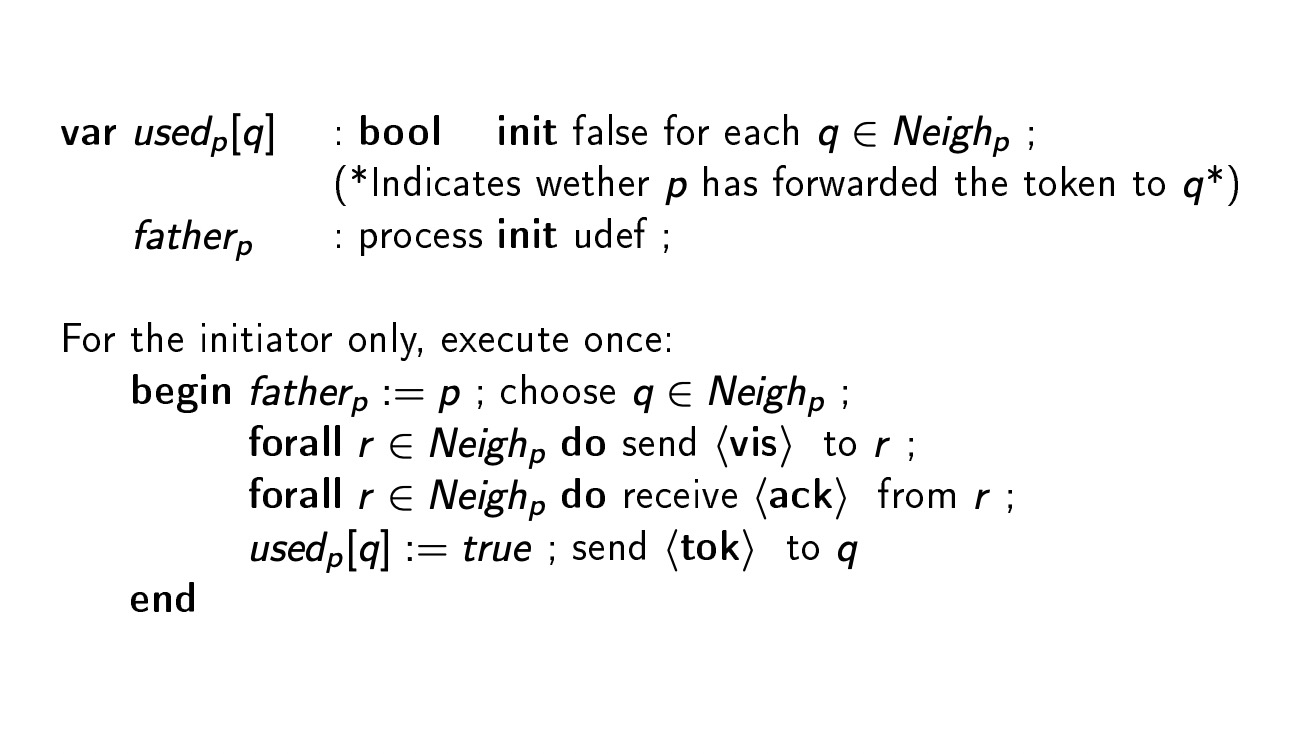
\includegraphics[width=0.8\textwidth]{figures/awerbuch1.jpg}
\end{figure}
\end{frame}

\begin{frame}
\begin{figure}
    \centering
    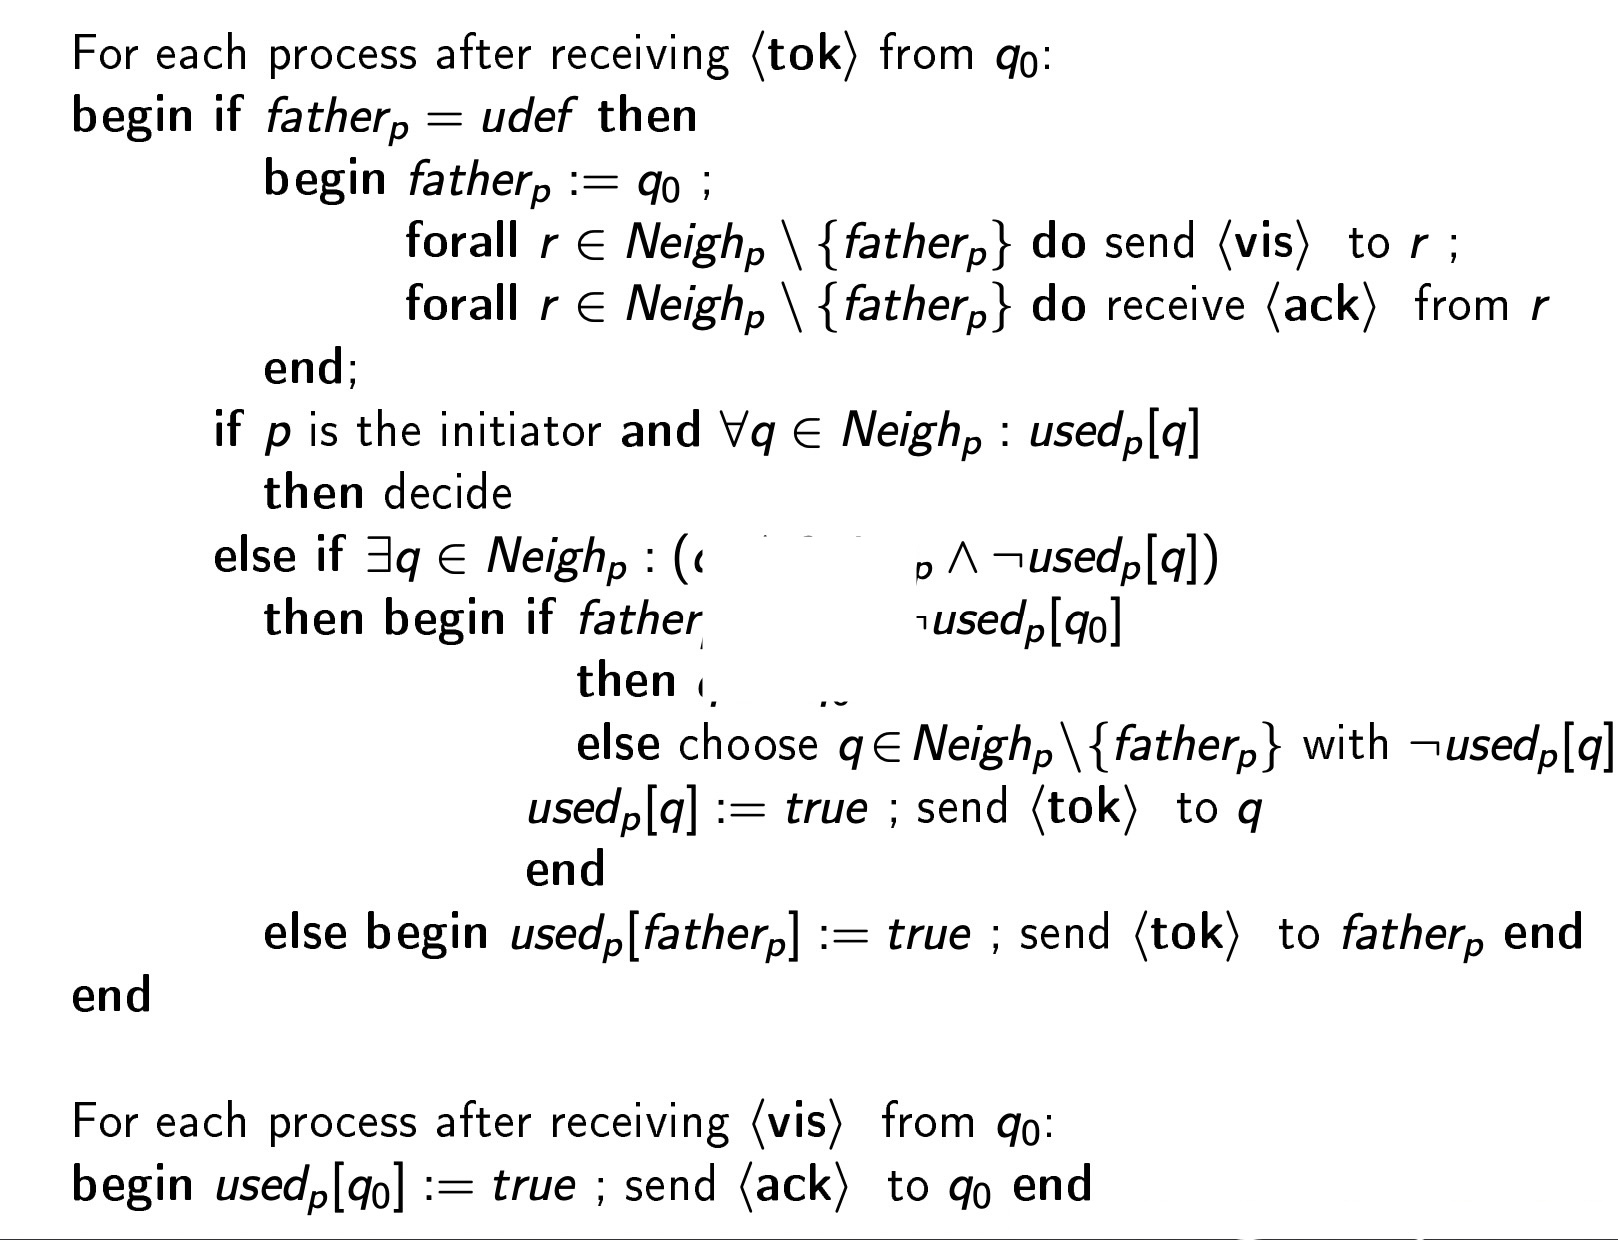
\includegraphics[width=0.8\textwidth]{figures/awerbuch2.jpg}
\end{figure}
\end{frame}


\subsection{Implementation}
\begin{frame}{Wave Traversal}
\framesubtitle{Cidon's DFS Algorithm}
The implementation of Cidon's DFS algorithm is based on the following key components:
\begin{itemize}
  \item Initialization: The initiator process sends a start message to its neighboring processes to begin traversal.
  \item Traversal Logic: Each process selects an unvisited neighbor to visit next and sends it a visit message.
  \item Acknowledgment: Cidon's algorithm eliminates the acknowledgment messages, reducing the communication overhead.

\end{itemize}

\end{frame}

\subsection{Algorithm}

\begin{frame}
\frametitle{Wave Traversal}
\framesubtitle{Cidon's DFS Algorithm}
Cidon's DFS algorithm shares similarities with Awerbuch's approach but streamlines the traversal process by eliminating the wait for acknowledgment messages.
 Upon receiving the start message, each process selects an unvisited neighbor and proceeds with traversal without waiting for acknowledgments.
 This design simplifies the algorithm and reduces traversal overhead, improving efficiency in distributed systems.
 While termination conditions may still involve waiting for traversal completion, the absence of acknowledgment messages enhances scalability and performance, making Cidon's algorithm an attractive choice for DFS traversal in distributed environments.
\end{frame}

\begin{frame}
\begin{figure}
    \centering
    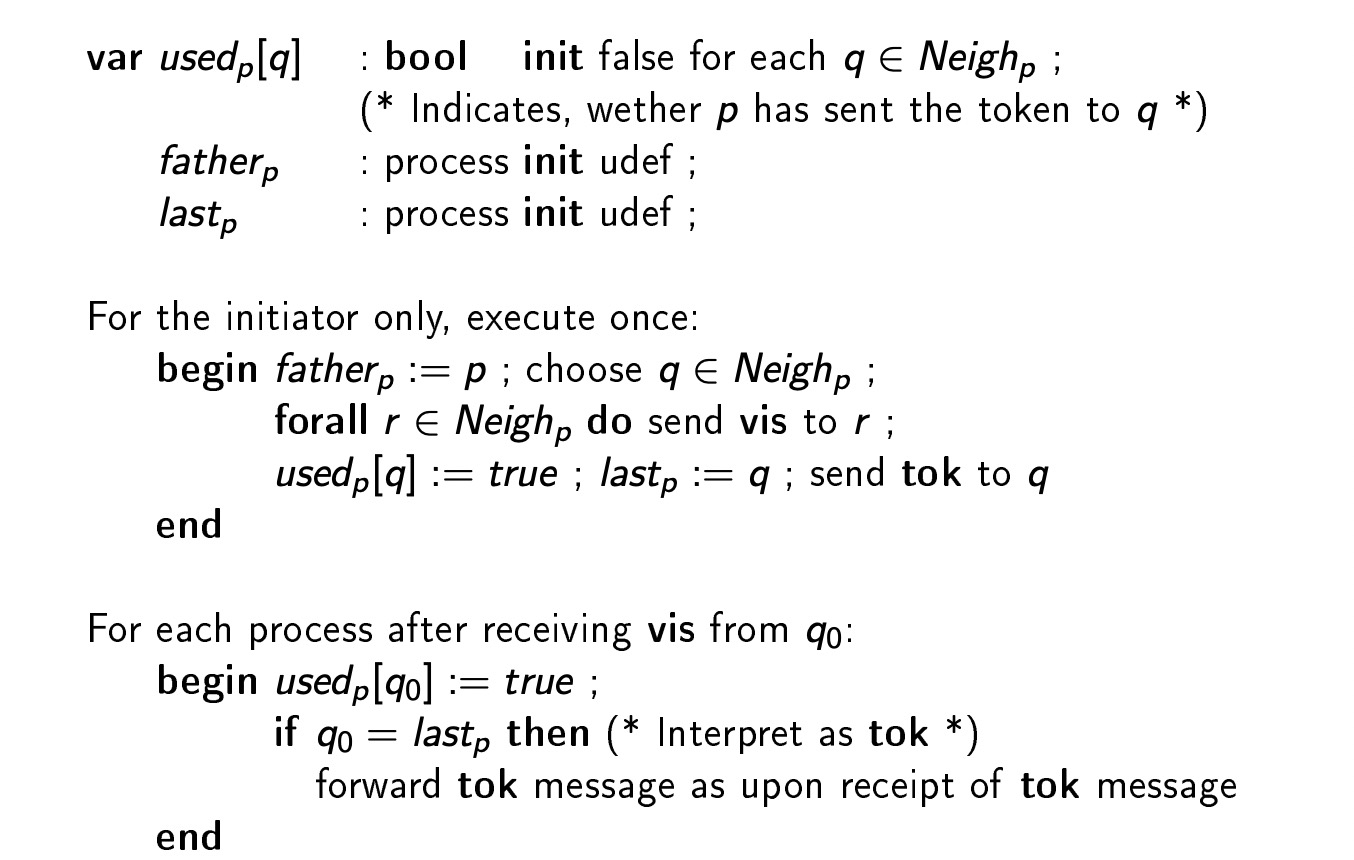
\includegraphics[width=0.8\textwidth]{figures/cidon1.jpg}
\end{figure}
\end{frame}

\begin{frame}
\begin{figure}
    \centering
    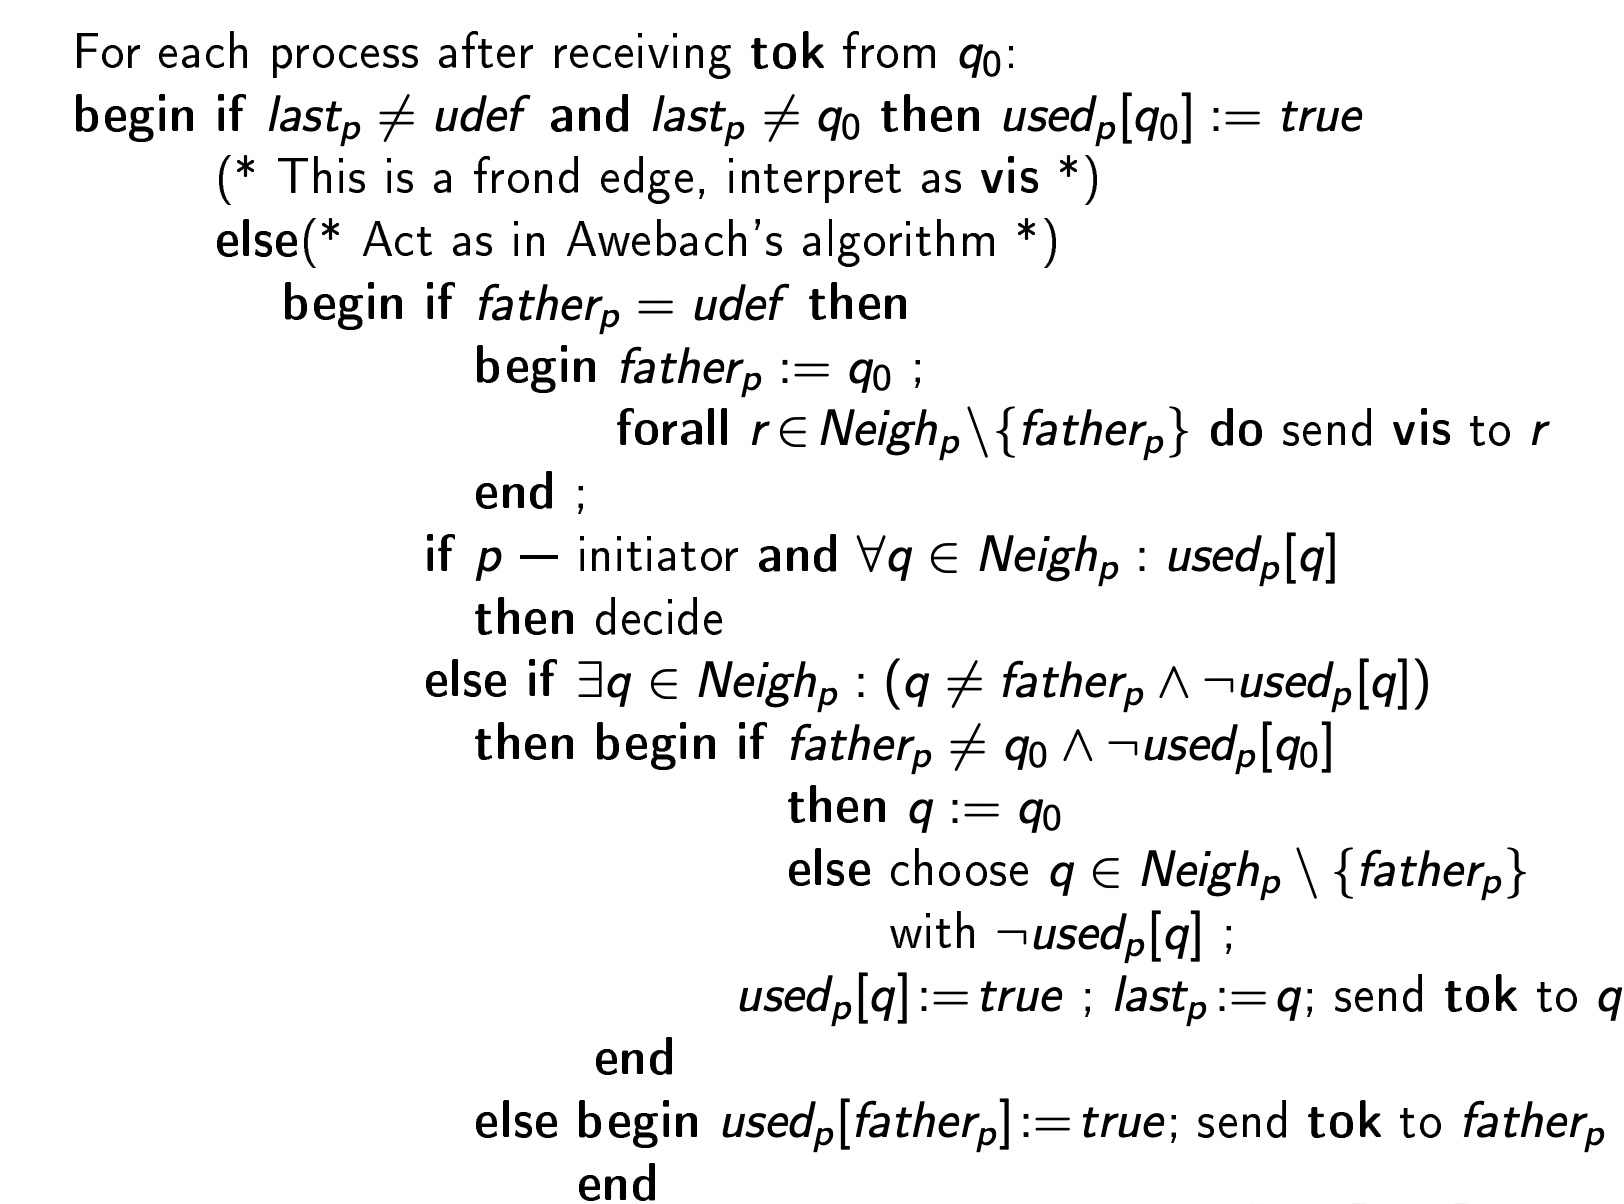
\includegraphics[width=0.8\textwidth]{figures/cidon2.jpg}
\end{figure}
\end{frame}

\section{Conclusions}
\begin{frame}
\frametitle{Conclusions}
\framesubtitle{Wave Traversal Algorithms in Distributed Systems}
\begin{itemize}
    \item Through testing is not done yet but the expected results are linear increase in message complexity and time complexity  with the number of nodes.
    \item Moreover, Cidon's Algorithm is expected to have better performance in terms of message complexity and time complexity compared to Awerbuch's Algorithm. Because it reduces the number of messages and does not wait for acknowledgment messages.
    \item Future work includes testing the algorithms in various network topologies and configurations to evaluate their performance and scalability.
\end{itemize}

\end{frame}

\section*{References}
\begin{frame}{References}
%\tiny
\bibliographystyle{IEEEtran}
\bibliography{refs}
\nocite{*} % used here because no citation happens in slides
\end{frame}


\thankslide

\end{document}